% -*-cap2.tex-*-
% Este fichero es parte de la plantilla LaTeX para
% la realización de Proyectos Final de Carrera, protegido
% bajo los términos de la licencia GFDL.
% Para más información, la licencia completa viene incluida en el
% fichero fdl-1.3.tex

% Copyright (C) 2009 Pablo Recio Quijano 

\section{Implementación}

Una vez terminadas las dos fases previas --- análisis y diseño --- es hora de enfrentarnos a la codificación e implementación
en sí de la aplicación. Este apartado es largo y entretenido, ya que va descubriendo a cada momento nuevas problemáticas que
no se han tenido en cuenta antes y es necesario resolver, pero también es apasionante, porque vamos viendo de forma
empírica cómo nuestra aplicación va tomando forma y se va haciendo tangible a cada momento que avanza. \\

El desarrollo de Dominous ha presentado muchas características interesantes, problemas, dificultades y otras circunstancias
que creemos interesante destacar, y que se pasamos a comentar a continuación.

\subsection{Entorno gráfico}

El entorno gráfico se puede dividir en dos apartados de diferente complejidad: por un lado tenemos la gestión de menús,
opciones, pantallas y secciones de la aplicación, y por otro lado tenemos la gestión de una partida de dominó, con todas
sus interacciones, animaciones y movimientos de fichas, eventos y demás.

\subsubsection{Sistema de secciones}

Todo el sistema de secciones lo gobierna el objeto principal de la aplicación, llamado \textbf{dominous}. Este objeto posee
diferentes objetos como atributos, y estos atributos son las diferentes secciones de la aplicación. Cuando queremos
que el flujo de la aplicación pase de una sección a otra no tenemos más que llamarla; al llamarla estaremos ejecutando
el siguiente fragmento:

\begin{lstlisting} [caption={Código Python de cambio de sección}, language=Python, numbers=left]
def goto_tutorial(self):
    self.flow.stop()
    self.flow = self.tutorial
    self.flow.start()
\end{lstlisting}

Gracias a este tipo de llamadas podemos subdividir cómodamente la aplicación en módulos muy acotados, a los cuales se aplica
primero una función de inicialización --- por si es necesario que actualicen estructuras, datos o cualquier otra labor
de preparación que puedan requerir --- y una vez se termina también se ejecuta una función de finalización. \\

Y mientras el flujo esté asociado a una sección, todas las funciones de eventos, dibujado y actualización de la pantalla
se disparan dentro de la sección correspondiente. \\

Gracias a esta metodología hemos podido acotar de forma muy cómoda las diferentes secciones (cada una con sus peculiaridades)
y gestionar de forma independiente cada apartado, evitando posibles problemas colaterales, asegurando una buena
integración y minimizando el hecho de que errores de un apartado puedan afectar a otros.

\subsubsection{Gestión de partida}

La gestión de la partida se puede dividir en dos apartados principales. El primero de ellos es la gestión de los diferentes
estados y transiciones en los que se divide la partida, y el segundo es el motor gráfico en sí, que dibuja y mueve
las fichas, el tablero y todos los diferentes elementos interactivos que incluye el juego. \\

La gestión de estados se ha programado con una máquina finita de estados --- o autómata finito --- ya que este tipo de
juegos por turnos se controla de forma cómoda y fácil con este tipo de estructuras. Contamos con un atributo \textbf{status}
de la clase principal; este estado se va comprobando y actualizando en los diferentes estados, tal y como se ve en la
estructura siguiente:

\begin{lstlisting} [caption={Autómata finito de estados}, language=Python, numbers=left]
"""
Status = 0 - game start, reset all, create players
    1 - fade in
    2 - deal tiles
    if game is over:
        999 - end game, goto menu
    if hand is over:
        99 - end hand
        100 - move tiles to center
        101 - show full screen scoreboard
        goto 1
    else:
        3 - draw available positions
        4 - ask tile next player
        if next player is human:
            if player must pass:
                20 - human player must pass
                21 - waiting to click pass button
                22 - human pressed pass button
                23 - pass effect
                goto 5
            else:
                6 - start drag n drop player tile
                7 - dragging tile
                8 - mousedown released
                if player can place tile here:
                    goto 5
                else:
                    goto 6
        else:
            if computer must pass:
                23 - pass effect
            else:
                5 - move tile to its place
            goto 3
"""
\end{lstlisting}

Así, siguiendo este diagrama de flujo con las posibles transiciones entre los diferentes estados, podemos definir y acotar
los posibles movimientos que se llevan a cabo a lo largo de la partida. \\

Por otro lado, el motor gráfico que participa de la partida consta de varios apartados y, probablemente, uno de los más costosos y
laboriosos fue el del método que decide en qué lugar se coloca una ficha en el tablero. \\

Como vemos en el gráfico~\ref{fig:tiles-position} existen multitud de posiciones y orientaciones posibles a la hora de colocar
la nueva ficha --- hasta un total de 20 diferentes posiciones, dependiendo de las siguientes variables:
\begin{itemize}
    \item Naturaleza de la ficha que vamos a colocar --- recordemos que las fichas dobles se colocan de forma
            perpendicular al sentido del flujo de las fichas, mientras que las fichas que no son dobles continúan con
            el sentido de las fichas.
    \item Orientación de la ficha de enganche.
    \item Sentido de las fichas en el tablero.
    \item Posición de la ficha de enganche en el tablero respecto a los límites del mismo.
    \item Número de fichas colocadas en el tablero --- si estamos colocando la primera ficha, esta debe situarse en
            el centro justo del tablero.
    \item Tamaño de las fichas y del área de juego.
\end{itemize}

\begin{figure}[h]
  \begin{center}
    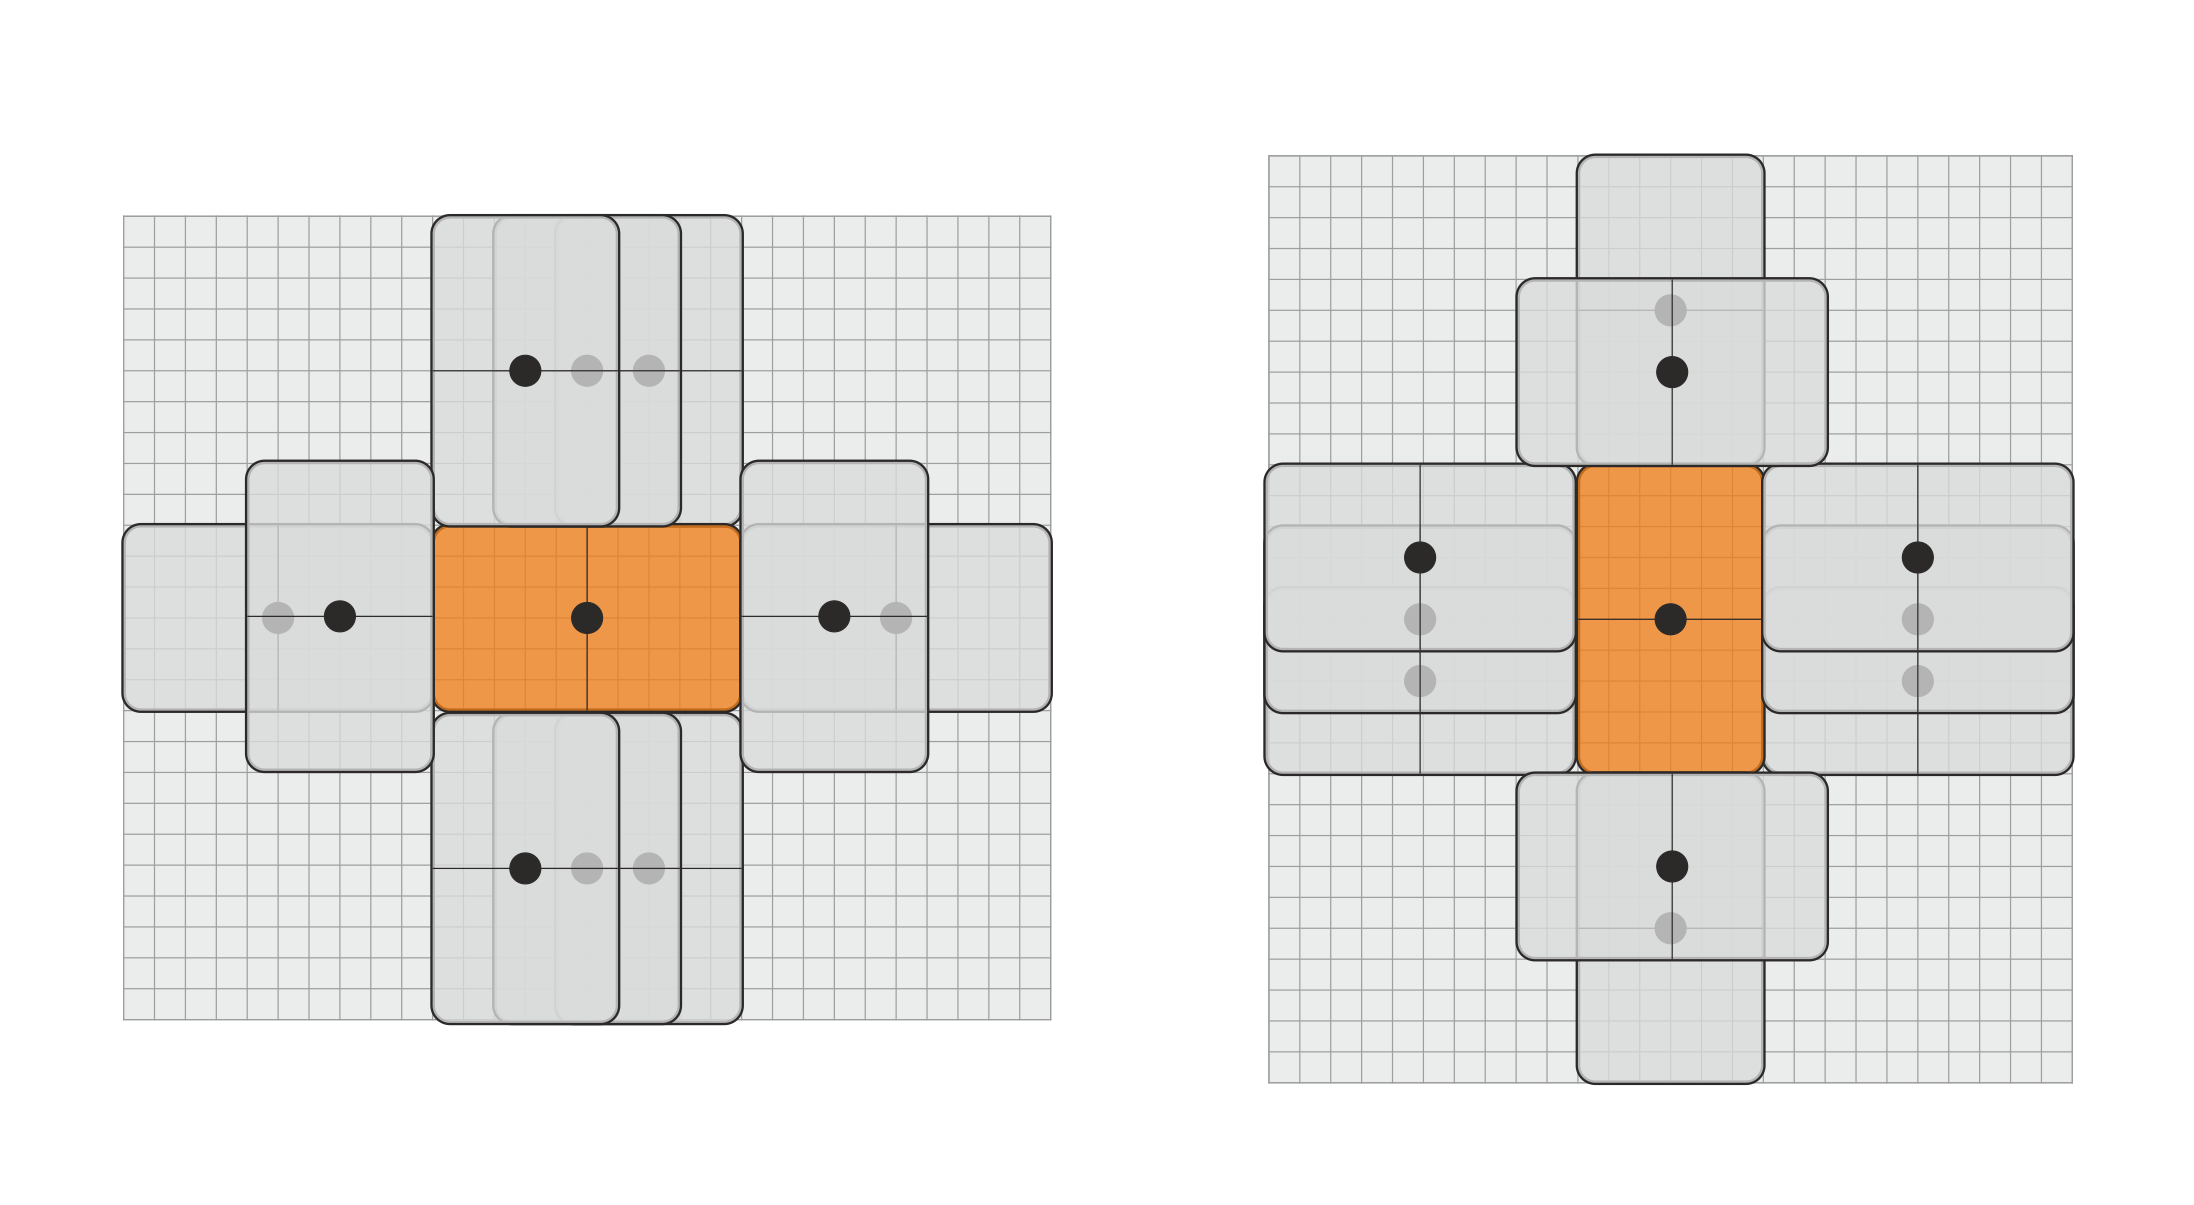
\includegraphics[scale=0.9]{tiles_position.png}
  \end{center}
  \caption{Diferentes posiciones en las que se puede colocar una ficha en el tablero}
  \label{fig:tiles-position}
\end{figure}

Para saber dónde colocar las fichas se necesita información de todas estas variables, y dependiendo del caso, optar por
una posición u otra. Dado que existen multitud de circunstancias y posibles opciones, se decidió encapsular en un método
y realizar todos los cálculos y comprobaciones para luego mover directamente la ficha.

\subsection{Interfaz de sonido}

La interfaz de sonido se ha diseñado de tal forma que se gestione de forma independiente para que su uso sea sencillo,
realizando llamadas al objeto \textbf{sound} con los métodos que estimemos oportunos en cada momento, y el propio
sistema se encarga de realizar diferentes cálculos y comprobaciones:

\begin{itemize} 
    \item Por ejemplo, a la hora de ejecutar un determinado fragmento musical, controla si ya se está escuchando música
        en ese momento; si es ese el caso realiza un pequeño fundido de la pista actual, e inicia la ejecución de la
        nueva, evitando así los desagradables clicks que se podrían escuchar cuando se para y se inicia la canción.
    \item O también, para ejecutar un sonido de ficha de dominó sobre el tablero, el sistema realiza la precarga de todos
        los sonidos --- similares pero no iguales --- y dispara uno aleatoriamente, evitando que cada apartado tenga
        que gestionarlo de forma autónoma
\end{itemize}


\subsection{Configuración de la aplicación}

La configuración de la aplicación (y almacenaje de la misma) se realiza mediante ficheros de tipo \textbf{INI}. Un archivo
INI consiste en un simple archivo de texto ASCII que contiene dos tipos de entradas:

\begin{description}
    \item[Secciones] permiten agrupar parámetros relacionados. Por ejemplo: "Parámetros de red".
    \item[Valores] definen parámetros y su valor. Primero se define el nombre del parámetro y después su valor separado por
            el signo de igualdad (=).
    \item[Comentarios] permiten explicar el propósito de una sección o parámetro. Los comentarios comienzan con el carácter
            punto y coma (;).
\end{description}

El significado de secciones y valores no está bien definido y cada aplicación puede reaccionar de manera diferente ante:

\begin{itemize}
    \item Secciones duplicadas.
    \item Parámetros duplicados.
    \item El carácter de barra invertida (\textbackslash). A veces se usa para romper una línea en dos.
    \item Valores. Los valores pueden consistir en texto, números, listas separadas por comas, etc. Esto depende de la aplicación.
\end{itemize}

Las ventajas de este tipo de ficheros es su estandarización y comodidad a la hora de leer y guardar valores en fichero,
de tal forma que podemos guardar información por defecto sobre el juego de la siguiente forma:

\begin{lstlisting} [caption={Fichero INI de ejemplo}, language=Python, numbers=left]
config.add_section('General')
config.set('General', 'name', 'Dominous')
config.set('General', 'window_caption', 'Dominous')
config.set('General', 'lang', 'en')
config.set('General', 'points_per_game', '200')
config.add_section('Screen')
config.set('Screen', 'window_width', '800')
config.set('Screen', 'window_height', '600')
config.set('Screen', 'full_screen', 'False')
config.set('Screen', 'window_fav', os.path.join('images', 'fav.png'))
config.add_section('Theme')
config.set('Theme', 'theme', 'spanish')
config.add_section('Game')
config.set('Game', 'player2', 'easy')
config.set('Game', 'player3', 'easy')
config.set('Game', 'player4', 'easy')
# write our configuration file to file
with open(file, 'wb') as configfile:
    config.write(configfile)
\end{lstlisting}

Y más tarde leerlo simplemente con:

\begin{lstlisting} [caption={Código Python de lectura de fichero INI},language=Python, numbers=left]
config = ConfigParser.RawConfigParser()
config.read(file)
config_default = {
    'name': config.get('General', 'name'),
    'window_caption': config.get('General', 'window_caption'),
    'window_width': config.getint('Screen', 'window_width'),
    'window_height': config.getint('Screen', 'window_height'),
    'full_screen': config.get('Screen', 'full_screen'),
    'window_favicon': config.get('Screen', 'window_fav'),
    'tile_width': 525,
    'tile_height': 270,
    'scale': 0.2,
    'theme': config.get('Theme', 'theme'),
    'lang': config.get('General', 'lang'),
    'points_per_game': config.get('General', 'points_per_game'),
    'gametype': 'human',
    'gametype_current': 'single',
    'player1': 'easy',
    'player2': 'easy',
    'player3': 'easy',
    'player4': 'easy',
    'speed': '1',
}
\end{lstlisting}

Todo ello encapsulado dentro del módulo \textbf{config.py} de la aplicación.

Con esto conseguimos un sistema para almacenar la configuración del sistema mediante un método portable, cómodo, sencillo y 
editable por el usuario mediante cualquier tipo de editor de texto (en caso de que existiera cualquier tipo de problema).

\subsection{Inteligencia Artificial}

En Dominous, el Sistema Experto de Inteligencia Artificial se reparte entre varios módulos, simplificando la implementación
de las diferentes partes. Según la estructura clásica en las que se divide un Sistema Experto, podemos ver que cada
apartado genera información o conocimiento para la Inteligencia Artificial:

\begin{description}
    \item[Base de conocimientos] Contiene conocimiento modelado extraído del diálogo con un experto --- Esta base de
        conocimiento se almacena, por un lado en la biblioteca de funciones y herramientas para desempeñar una partida,
        y físicamente se almacena en el módulo de IA
    \item[Base de hechos (Memoria de trabajo)] Posee los hechos sobre un problema que se ha descubierto durante el análisis
        --- Los hechos se van creando y almacenando gracias al módulo de \textbf{Gestión de Partida de Dominó}, que
        gobierna la partida y guarda toda la información, movimientos, pasos y tiempos al colocar las fichas.
    \item[Motor de Inferencia] Modela el proceso de razonamiento humano --- gracias a la biblioteca de funciones podemos
        crear un motor de inferencia fácilmente, utilizando pequeñas reglas y dotando de peso o importancia a cada una,
        modelando exactamente el proceso de razonamiento que queramos, e incluso ofertando la posibilidad de crear
        cuantos queramos, de una forma fácil y rápida.
    \item[Módulos de justificación] Explica el razonamiento utilizado por el sistema para llegar a una determinada conclusión
        --- ya que en el dominó no se puede evaluar por sí mismo la efectividad o conveniencia de un movimiento, esta
        justificación llega del conocimiento del experto en valorar con mayor o menor peso una regla.
    \item[Interfaz de usuario] Esta última capa es la interacción entre el Sistema Experto y el usuario, se realiza
        mediante el lenguaje natural --- y, en el caso de Dominous, la interfaz se comunica con el usuario mediante el
        módulo del motor gráfico del juego, que muestra fichas, movimientos y jugadores.
\end{description}

Pasemos a describir cada apartado para conocer a fondo la implementación del sistema experto.

\subsubsection{Base de conocimientos}

La base de conocimiento se obtiene desde el módulo \textbf{Gestión de Partida de Dominó}, que almacena la información
de forma global, esto es, relativa a toda la partida:

\begin{lstlisting} [caption={Información global de la partida}, language=Python, numbers=left]
self.info = {
    "date" : date,
    "place" : place,
    "max_points" : max_points,
    "player1" : player1,
    "player2" : player2,
    "player3" : player3,
    "player4" : player4,
    "team1" : player1 + " " + player3,
    "team2" : player2 + " " + player4,
    "description" : description,
    "winner_team" : "",
    "team1_points" : 0,
    "team2_points" : 0,
}
\end{lstlisting}

Como vemos, el identificador de cada campo es bastante descriptivo, añadiéndose mucha información complementaria que pueda
necesitarse en un futuro. \\

El sistema también almacena información de la mano actual y de cada movimiento de la siguiente forma:

\begin{lstlisting} [caption={Información de la mano actual}, language=Python, numbers=left]
movement = {
    'player' : player,
    'tile' : tile,
    'side' : side,
    'left' : left,
    'right' : right,
    'mtime' : mtime,
}
\end{lstlisting}

Entre los campos almacenados vemos uno que nos resultará de mucho interés en posteriores usos de esta información, y es
el campo \textbf{mtime}. Este campo almacena el tiempo que ha estado el jugador pensando antes de colocar una ficha,
y gracias a que el dominó es un juego de caballeros podemos utilizar esta información para elaborar una estrategia
para conseguir la victoria. \\

Los posibles valores que puede presentar este campo son:

\begin{description}
    \item[0] El usuario no ha requerido tiempo para decidir qué ficha colocaba.
    \item[1] El usuario ha pensado entre diferentes opciones, y ha necesitado de cierto tiempo para decidir la ficha.
    \item[2] El usuario ha utilizado una cantidad de tiempo considerable para decidir la ficha a colocar.
\end{description}

\subsubsection{Base de Hechos}

La Base de Hechos se ha modularizado en pequeñas funciones o reglas, de tal forma que pueden ser fácilmente reutilizadas en
el Sistema Experto de cualquier jugador de Dominous. La estructura básica de una regla es la siguiente:

\begin{lstlisting} [caption={Estructura básica de regla}, language=Python, numbers=left]
class nombre_de_la_regla:
    def __init__(self):
        # inicializamos los atributos que sean necesarios
        pass
    def go(self, left_tile, right_tile, board, tiles, log):
        return ficha, lado, tiempo_pensando
\end{lstlisting}

Como vemos la estructura es sencilla, implementada mediante clases Python, y tiene una inicialización para definir los
atributos que sean necesarios, y por otra parte un método que, para una situación concreta de estado de la partida
(tablero, fichas propias, posición del jugador y toda la información generada por la partida). \\

Veamos un ejemplo práctico. Vamos a definir una regla que intente colocar sobre el tablero una ficha doble, cualquiera
que tengamos. Esta regla se implementaría de la siguiente forma:

\begin{lstlisting} [caption={Regla para colocar ficha doble}, language=Python, numbers=left]
class put_any_double:
    def __init__(self):
        pass
    def go(self, left_tile, right_tile, board, tiles, log):
        for item in tiles:
            if item[0] == item[1]:
                if item[0] == left_tile or item[1] == left_tile:
                    tiles.remove(item)
                    return item, "left", 1
                    break
                elif item[0] == right_tile or \
                    item[1] == right_tile or \
                    left_tile == None:
                    tiles.remove(item)
                    return item, "right", 1
                    break
        return None, "pass", 0
\end{lstlisting}

En la inicialización no requerimos dar de alta ningún atributo, y el método \textbf{go} simplemente comprueba que, para
alguna de nuestras fichas dobles, algún lado de la mesa tenga ese mismo valor. Si lo tiene hemos conseguido realizar
esta regla, devolvemos el valor y listo. Y si no, devolvemos una señal de que no hemos tenido éxito y salimos. \\

Gracias a este sistema, simplificamos mucho el desarrollo de nuevos Sistemas Expertos, ya que:
\begin{itemize}
    \item Es muy sencillo crear nuevas reglas. Como ya vimos en El Libro del dominó de Benito Ruipérez \cite{mora90},
        muchas reglas, funciones o herramientas se basan en frases o hechos que, si se cumplen, \emph{interesa}
        \footnote{Como vemos, debemos ser cuidadosos al emplear verbos como \emph{interesa} o \emph{debemos} al hablar
        de colocar fichas. El juego del Dominó es lo suficientemente complejo y goza de muchas estrategias como para poder
        simplificarlo o decir objetivamente que debemos realizar una acción.} cumplirlos.
        Por poner un caso simple, al comenzar la partida \emph{interesa} comenzar con un doble --- o, mejor dicho, hay
        estrategias interesadas en comenzar con un doble. Para emplear este razonamiento en estas estrategias simplemente
        tenemos que añadir esta regla con el peso suficiente, y ya lo tendremos implementado.
    \item Es fácil crear nuevos sistemas, creando pilas de reglas con pesos que se van disparando si pueden cumplirse.
        Así se van creando diferentes jugadores y dotamos al juego de más variedad y diversión.
\end{itemize}

Los jugadores poseen una lista de elementos, utilizando normalmente la nomenclatura \textbf{self.knowledge}, y van
añadiendo las reglas que estimen oportunas como si fuera una lista clásica de Python, utilizando el método \textbf{append}. \\

Si estamos desarrollando un jugador simple, podemos definir su base de conocimiento de la siguiente forma:

\begin{lstlisting} [caption={Base de conocimiento simple}, language=Python, numbers=left]
self.knowledge = []
self.knowledge.append([put_any_double()])
self.knowledge.append([put_anyone()])
\end{lstlisting}

Como vemos, estamos definiendo que el jugador intente, inicialmente, colocar una ficha doble. Si esto no es posible,
intentará colocar una ficha cualquiera. \\

Así, con solamente tres líneas podemos comenzar a desarrollar una inteligencia artificial a nuestro gusto, que juegue
y valore cada regla con la importancia que estimemos oportuna. \\

Por otro lado, también podemos utilizar reglas con el mismo peso, dotando de aleatoriedad al jugador y permitiendo
que se comporte de diferente modo en situaciones similares. De este modo, si queremos definir a un jugador un poco
más complejo, su base de conocimiento podría escribirse así:

\begin{lstlisting} [caption={Base de conocimiento compleja}, language=Python, numbers=left]
self.knowledge = []
self.knowledge.append([
    put_any_double(),
    weight_matrix()
])
self.knowledge.append([put_anyone()])
\end{lstlisting}

En un primer momento se ejecutará, aleatoriamente, una regla entre \textbf{put\_any\_double()} y \textbf{weight\_matrix()}.
Si no hay suerte con la primera, se intentará con la segunda, y si no hay éxito con ninguna se ejecutará el siguiente
conjunto de reglas --- en este caso, \textbf{put\_anyone()}, es decir, intentar colocar una ficha cualquiera.

El Motor de Inferencia se desarrolla de forma muy sencilla, ya que se utilizan estructuras muy simples proporcionadas
por el mismo lenguaje Python. \\

\subsubsection{Motor de Inferencia}

El Motor de Inferencia es el encargado de elegir una regla de entre todas las reglas definidas en la Base de Conocimiento
del jugador concreto. Este motor, antes de evaluar cualquier regla, realiza diferentes comprobaciones para acelerar
los tiempos de cálculo en ciertos casos especiales. Así, las reglas no se evaluarán bajo las siguientes circunstancias:
\begin{itemize}
    \item El jugador no puede colocar ninguna ficha --- si ninguna de las fichas que posee el jugador son candidatas
        a utilizarse en el tablero, el Motor de Inferencia pasará automáticamente el turno al siguiente jugador.
    \item El jugador solo puede colocar una ficha ---  en el caso de que solamente una ficha sea candidata a colocarse
        en juego, el sistema la colocará automáticamente, dando la información de que el jugador ha estado poco tiempo
        pensando qué ficha colocar, y pasará el turno al siguiente jugador.
\end{itemize}

Solamente en el caso de que más de una ficha sea candidata a colocarse, el Motor de Inferencia hará uso de la Base
de Conocimiento y aplicará las reglas del sistema experto.

\subsection{Música y efectos}

La música también juega un papel importante en un videojuego, y no debe ser elegida a la ligera, sino
        debe buscarse una razón y un estilo que encaje con los objetivos definidos. Esta aplicación está orientada a un
        público muy general, y el ritmo del juego es tranquilo y pausado, así que se eligió el jazz como estilo base
        para acompañar al juego. \\

\begin{figure}[h]
  \begin{center}
    
\includegraphics[scale=0.8]{jamendo.jpg}
  \end{center}
  \caption{La música se obtuvo de Jamendo, un servicio de música libre}
  \label{jamendo}
\end{figure}

        Gracias a la enorme comunidad de músicos que publican sus obras con \emph{licencias libres}
        --- permitiendo que sus obras se utilicen y se adapten a otros entornos --- no fue nada complicado buscar
        un conjunto de canciones que se adaptaran al ritmo y velocidad que se disfruta en Dominous. \\

        En cuanto a los efectos de sonido la cosa estuvo un poco más complicada. Al inicio se buscaron sonidos que
        pudieran encajar con las acciones de colocar la ficha, y se probó con efectos de sonido clásicos de click --- sonidos
        cortos que informan de una acción --- pero se descubrió que, aunque dotaban de la suficiente información
        al usuario, no quedaban bien con la estructura y estilo de Dominous. \\

        La solución que se tomó fue grabar sonidos reales de fichas de dominó golpeando una mesa. Una vez se contó con
        un buen grupo de sonidos, se eligió uno como candidato un golpe seco, limpio y con sonoridad. Pero descubrimos
        que escuchar siempre el mismo sonido era molesto para el usuario (y muy poco realista), así que se optó por mejorar
        la solución final: elegir un gran conjunto de sonidos diferentes de fichas de dominó y ejecutar aleatoriamente
        uno de ellos cada vez que la ficha golpeaba la mesa. \\
        
        Tras tratar estas muestras con un software de edición de sonidos~\cite{IPalomo} conseguimos una sonoridad y aleatoriedad agradable para el usuario.
